\chapter{Methodology}
\section{Outline}
This section will look into the mechanical design of the Stewart platform, considerations for the force sensor and the velocity measurement within the wind tunnel. It will finally look into the design of a human machine interface that will be used to control the Stewart platform, obtain measurements and display results.

\section{Design of Stewart Platform}
This section deals with: design considerations, position, velocity and acceleration analysis of the Stewart platform.
\subsection{Design Considerations}
\begin{enumerate}
\item When the controllable axes are active, the platform must be controlled in six degrees of motion.
\item When the controllable members are stationary, the
platform must have a corresponding fixed position.
\item The design parameters for consideration are: mobile platform radius, height of the platform and angle between adjacent joints of mobile platform and base plate.
\item The mechanism should be lightweight.
\item Velocity and position control of the mechanism should be easy to achieve.
\end{enumerate}
\subsection{Kinematic Analysis - Rotational matrix}
Euler angles are utilized to obtain rotational matrix for the moving platform of the Stewart platform mechanism. The rotational matrix is represented as follows \cite{csumnu2017simulation}:
\begin{equation}
 R_{P}^B = R_{Z}(\gamma)*R_{Y}(\beta)*R_{X}(\alpha)
\end{equation}
Where $\gamma, \beta, \alpha$ - angles of rotation about the z-, y- and x-axis respectively.

In matrix form:
\[ R_{P}^B =
 \begin{bmatrix}
 c\beta c\gamma & s\alpha s\beta c\gamma - c\alpha s\gamma & c\alpha s\beta c\gamma + s\alpha s\gamma\\
 c\beta s\gamma & s\alpha s\beta s\gamma + c\alpha c\gamma & c\alpha s\beta s\gamma - s\alpha c\gamma\\
 -s\beta & s\alpha c\beta & c\alpha c\beta  
 \end{bmatrix}
\]
Generalized coordinate position and velocity vector of the moving platform is represented below \cite{csumnu2017simulation}:
\[
q=
\begin{bmatrix}
tx & ty & tz & \alpha & \beta & \gamma
\end{bmatrix}^\top
\]
\[
\dot{q}=
\begin{bmatrix}
\dot{tx} & \dot{ty} & \dot{tz} & \dot{\alpha} & \dot{\beta} & \dot{\gamma}
\end{bmatrix}^\top
\]
Transformation of angular velocity of moving platform to the base frame can be done using Euler angles \cite{csumnu2017simulation}:
\[
\omega =
\begin{bmatrix}
1 & 0 & s\beta \\
0 & c\alpha & -s\alpha c\beta \\
0 & s\alpha & c\alpha c\beta 
\end{bmatrix}
\begin{bmatrix}
\dot{\alpha} \\
\dot{\beta}\\
\dot{\gamma}
\end{bmatrix}
\]
Acceleration of the moving platform is obtained by differentiating the velocity of the moving platform with respect to time:
\[
\dot{\omega} =
\begin{bmatrix}
1 & 0 & s\beta \\
0 & c\alpha & -s\alpha c\beta \\
0 & s\alpha & c\alpha c\alpha c\beta 
\end{bmatrix}
\begin{bmatrix}
\ddot{\alpha} \\
\ddot{\beta}\\
\ddot{\gamma}
\end{bmatrix}
+
\begin{bmatrix}
0 & 0 & \dot{\beta}c\beta \\
0 & \dot{\alpha} s\alpha & -\dot{\alpha} c\alpha c\beta + s\alpha \dot{\beta} s\beta \\
0 & \dot{\alpha}c\alpha & -\dot{\alpha}s\alpha c\beta - c\alpha \dot{\beta}s\beta
\end{bmatrix}
\begin{bmatrix}
\dot{\alpha} \\
\dot{\beta}\\
\dot{\gamma}
\end{bmatrix}
\]
\subsection{Inverse Kinematic Analysis}
Inverse kinematic analysis is used to determine the length of the legs according to planned trajectories of the moving platform position. In order to consider the length of the leg of a Stewart platform, closed-loop of one leg is used as shown in figure 3.1. Using this closed-form representation, the leg
vector with respect to base platform can be obtained as follows \cite{csumnu2017simulation}:
\begin{equation}
\label{eqn}
L_{i} = q_{i}^{B} - b_{i}
\end{equation}
The position vector of ith upper junction point with respect to the base frame is given by the following;
\begin{equation}
\label{eqn}
q_{i}^{B} = t + R_{p}^{B} * q_{i}^{p}
\end{equation}
\begin{center}
	\begin{figure}[H]
	\centering
	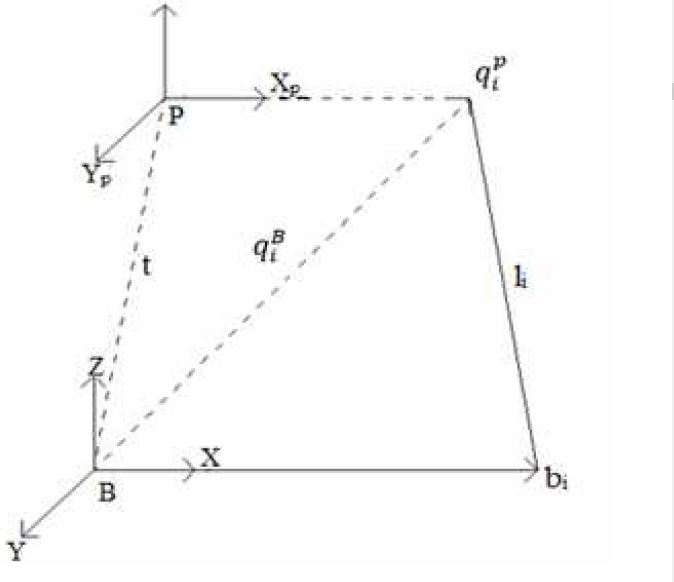
\includegraphics[width=0.6\linewidth]{Figures/Fig12}
	\caption[Closed-loop representation]{Closed-loop representation of one leg of the Stewart Platform \cite{csumnu2017simulation}}
	\end{figure}
\end{center}
Then the length of the ith leg can be acquired as follows:
\newpage
\begin{multline}
\label{eqn}
l_{i}^2 = (a_{x} * r_{p} * c_{i} + b_{x}*r_{p}*s_{i}
+ t_{x}-r_{b}*c_{i})^2 + \\(a_{y}*r_{p}*c_{i} + b_{y}*r_{p}*s_{i} + t_{y}-r_{b}*s_{i})^2+ (a_{z}*r_{p}*c_{i}+b_{z}*r_{p}*s_{i}+t_{z})^2
\end{multline}
%\subsection{Inverse Velocity Analysis}
%Inverse Jacobian matrix can be used to perform inverse velocity analysis of the Stewart
%platform. Inverse Jacobian matrix describes relation between velocity of the moving platform and the leg velocity.

%Inverse Jacobian matrix for a 6-DOF Stewart Platform
%\cite{csumnu2017simulation}:
%\[ J^-1 =
%\begin{bmatrix}
%u_{1}^{T} & (R_{P}^{B}q_{1}^{B} * u_{1})^T\\
%u_{2}^{T} & (R_{P}^{B}q_{2}^{B} * u_{2})^T\\
%u_{3}^{T} & (R_{P}^{B}q_{3}^{B} * u_{3})^T\\
%u_{4}^{T} & (R_{P}^{B}q_{4}^{B} * u_{4})^T\\
%u_{5}^{T} & (R_{P}^{B}q_{5}^{B} * u_{5})^T\\
%u_{6}^{T} & (R_{P}^{B}q_{6}^{B} * u_{6})^T
%\end{bmatrix}
%\]
\section{Base and Moving Platform}
 The Stewart platform should be stable. Thus the base will have a larger diameter than that of the moving platform. The Center of Gravity (COG) shouldn't fall outside the base during any of the platform movements.
\subsection{Stewart Platform Configurations}
Stewart platforms can take three primary configurations i.e. 3-3 type, 3-6 type or 6-6 type.
\begin{center}
	\begin{figure}[H]
	\centering
	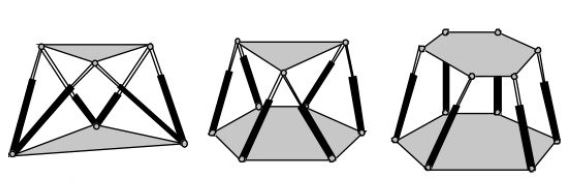
\includegraphics{Figures/stewart}
	\caption[Configurations]{Type 3-3, 3-6 and 6-6 respectively
	\cite{fernandes_design_nodate}}
	\end{figure}
\end{center}
The base and the platform (for the 3-3 type), and the platform (for the 3-6 type) are triangular in shape. The triangular shape has a good load carrying capability only in theory and for certain dimensions. These configurations are, however,not possible in practice since double spherical joints will be needed where two bars have to be joined at the same vertex
\cite{fernandes_design_nodate}.

Thus a 6-6 type platform is considered. The base and platform will be hexagon in shape.

\subsection{Quality Index $(\lambda)$ of Stewart Platform Design}
Quality index $(\lambda)$ varies from 0 to 1.\\
Where,\\
0 - design with singularities and\\
1 - Optimal design in which the determinant of the correspondent Jacobian matrix is maximum.

\textbf{Singularities} - uncontrollable states.

The Jacobian matrix relates the axial forces in the $i^{th}$ bar with the applied
forces and torques and is given in equation \eqref{eq:myeqn}:

\begin{equation}
J =
\begin{pmatrix}
\hat{\boldsymbol{S_{1}}} & \hat{\boldsymbol{S_{2}}} & \hat{\boldsymbol{S_{3}}} & ... & \hat{\boldsymbol{S_{n}}}
\end{pmatrix}
\label{eq:myeqn}
\end{equation}
Where n - number of bars and $ \hat{\boldsymbol{S_{i}}}$ - unit vector of the Plucker coordinates along the line of the
$i_{th}$ bar.

Quality index can be obtained as shown:
\begin{equation}
\lambda = \frac{|J|}{|J|_{m}}
\label{eq:myeqn}
\end{equation}
Where, $|J|$ is the determinant of the Jacobian matrix of a given Stewart platform configuration, and $ |J|_{m} $ - determinant of Jacobian Matrix of the optimal configuration.

Applying equation 3.3.1 to the general configuration of a 6-6 platform, it is
possible to obtain the Jacobian matrix and thus its determinant which can be obtained as in equation \eqref{eq:myeqn},
\begin{equation}
|J| =
\begin{pmatrix}
\frac{81 \sqrt{3} a^3 b^3 h^3 (3 \alpha \beta - 2 \alpha - 2 \beta +1)^3}{4(a^2(3 \alpha^2 - 3 \alpha + 1)+ ab(\alpha \beta - 1 )+ b^2(3 \beta^2 - 3 \beta + 1)+ 3h^2)^3}
\end{pmatrix}
\label{eq:myeqn}
\end{equation}
Where: a - diameter of moving platform
b - diameter of base
$\alpha$ - angle of attack
$ \beta $ - Side slip angle.
h - distance between the base and the moving platform.
$|J|_{m}$ is found by differentiating equation (3.3.3) with respect to h and equating to 0 resulting in \cite{fernandes_design_nodate}:
\begin{equation}
h = \sqrt{\frac{1}{3}(a^2 (3 \alpha^2 - 3 \alpha + 1)+ ab (3\alpha\beta - 1)+b^2(3 \beta^2 - 3 \beta + 1))}
\label{eq:myeqn}
\end{equation}
A base diameter of 300mm, platform diameter of 200mm and height of 190mm is considered.

For a = 200mm, b = 300mm, h = 190mm , $\alpha = 0.25$, $ \beta = 0.1667$,
\begin{equation}
|J| =
\begin{pmatrix}
\frac{81 \sqrt{3} a^3 b^3 h^3 (3 \alpha \beta - 2 \alpha - 2 \beta +1)^3}{4(a^2(3 \alpha^2 - 3 \alpha + 1)+ ab(\alpha \beta - 1 )+ b^2(3 \beta^2 - 3 \beta + 1)+ 3h^2)^3}
\end{pmatrix}
= 2.437 \times 10^-3
\label{eq:myeqn}
\end{equation}
And $ |J|_{m}$ where,
\begin{equation}
h = \sqrt{\frac{1}{3}(a^2 (3 \alpha^2 - 3 \alpha + 1)+ ab (3\alpha\beta - 1)+b^2(3 \beta^2 - 3 \beta + 1))} = 0.0764
\label{eq:myeqn}
\end{equation}
\begin{equation}
|J|_{m} =
\begin{pmatrix}
\frac{81 \sqrt{3} a^3 b^3 h^3 (3 \alpha \beta - 2 \alpha - 2 \beta +1)^3}{4(a^2(3 \alpha^2 - 3 \alpha + 1)+ ab(\alpha \beta - 1 )+ b^2(3 \beta^2 - 3 \beta + 1)+ 3h^2)^3}
\end{pmatrix}
= 2.834 \times 10^-3
\label{eq:myeqn}
\end{equation}
Quality index for this Stewart Platform design is therefore, 
\begin{equation}
\lambda = \frac{|J|}{|J|_{m}} = 0.86
\label{eq:myeqn}
\end{equation}
A quality index of 0.86 presents a design of high quality and mechanical feasibility.
\subsection{Sheet Metal Thickness and Material Selection}
Metal used to manufacture the base should be of significant thickness to provide more support to the whole structure.

Metal used to manufacture the moving platform should be lightweight and of enough thickness to enable it to withstand significant loads.

Some sheet metal materials are considered and compared.
\begin{table}[!h]
	\caption[Sheet Metal Properties]{Material Properties}
\end{table}
\begin{center}
\centering
\begin{tabular}{|l|l|l|}
\hline
\textbf{Metal} & \textbf{Density$(gcm^{-3})$} & \textbf{Yield Strength(MPa)}\\
\hline
Aluminium (6061-T6)& 2.7 & 270\\
\hline
Mild Steel & 7.85 & 250\\
\hline
Stainless Steel & 7.5 - 8.0 & 215\\
\hline
\end{tabular}
\end{center}
Aluminium 6061 is preferable for the moving platform since it is lightweight and can withstand significant loads without yielding. It also has good machinability (50 per cent). A sheet metal of 1.5mm thickness will make a suitable platform to be used in wind tunnel testing.
\begin{center}
	\begin{figure}[H]
	\centering
	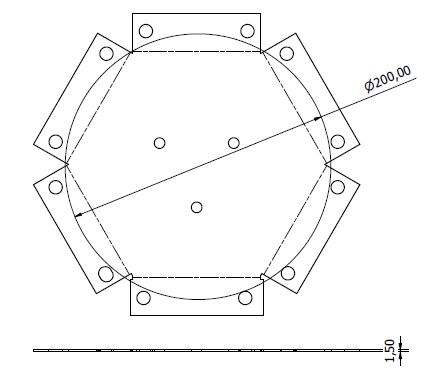
\includegraphics[width=0.6\linewidth]{Figures/Flat}
	\caption[Moving Platform]{Moving Platform (Flat Pattern)}
	\end{figure}
\end{center}

The moving platform has flanges to provide linking points of the Stewart Platform legs. A flange of 30mm is considered. This will allow ample space for the spherical joint (whose connecting side diameter is 10mm) to fit and to be well centred.
\begin{center}
	\begin{figure}[H]
	\centering
	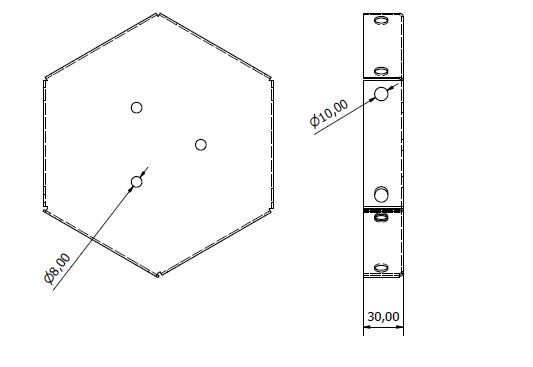
\includegraphics[width=0.6\linewidth]{Figures/Folded}
	\caption[Moving Platform]{Moving Platform (Folded)}
	\end{figure}
\end{center}

Both stainless steel and mild steel would make a suitable base for the Stewart platform due to their weight. They are also easy to machine (machinability for Mild steel - 78 per cent, for stainless steel: 45 - 110 per cent). Mild steel is readily available in the Kenyan market. Stainless steel is a bit more expensive.

Due to cost constraints and for the Stewart platform's overall weight (and without compromising on the platform stability), aluminium can be used to manufacture the base. A thickness of 2.5mm is selected.
\begin{center}
	\begin{figure}[H]
	\centering
	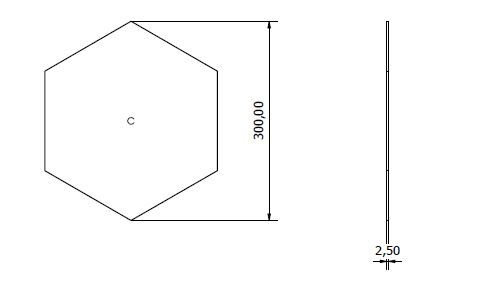
\includegraphics[width=0.6\linewidth]{Figures/Base}
	\caption[Base Plates]{Base Plates}
	\end{figure}
\end{center}
Aluminium, unlike mild steel, would not require post-processing methods (e.g. powder coating) which would add on the cost.
\section{Sensing Bars/Rods}
Two options are considered:
\begin{itemize}
\item Bars with square cross-section
\item Cylindrical bars
\end{itemize}
Cylindrical bars are selected due to their ease of coupling with the available spherical joints. Cylindrical bars also guarantee uniform deformation of the bars - both in the axial and cross-sectional directions.

From inquiries around suppliers in the Kenyan Market, these bars are usually available in steel and aluminium. In order to select the optimum solution for our application, the Yield Strength, modulus of rigidity, Young's Modulus and density of both materials will be considered. 
\begin{table}[!h]
\caption[Aluminium and Steel Properties]{Material Properties of Aluminium and Steel}
\end{table}

\begin{tabular}{|l|l|l|l|l|}
\hline
\textbf{Material} & \textbf{Yield Strength (MPa)} & \textbf{G (GPa)} & \textbf{E (GPa)} & \textbf{Density ($g/cm^3$)}\\
\hline
Steel & 240 & 79 & 190 - 215 & 7.8\\
\hline
Aluminium & 270 & 26 & 69 - 70 & 2.7\\
\hline
\end{tabular}

E - Young's Modulus\\
G - Modulus of Rigidity

From $ \sigma = E \epsilon $, where $\sigma$ - Stress , E - Young's Modulus and $ \epsilon$ - Strain, materials with high values of Young Modulus will give smaller values of strain when subjected to a deforming force. Thus, aluminium rods will experience higher strains than steel rods.

Materials with high modulus of rigidity will require huge amounts of force to deform. Aluminium rods will experience deformation under small amounts of force as compared to steel rods.

Aluminium rods have the capability of bearing higher loads before their deformation goes from elastic to plastic as compared to steel rods. Aluminium rods also have the benefit of being lightweight.

\subsection{Sensing Rods Design - Length}
From the previously selected dimensions i.e diameter of platform, diameter of base and distance between the base and platform, the length of each rod can be determined by geometry.

Rod length = 140mm
\begin{center}
	\begin{figure}[H]
	\centering
	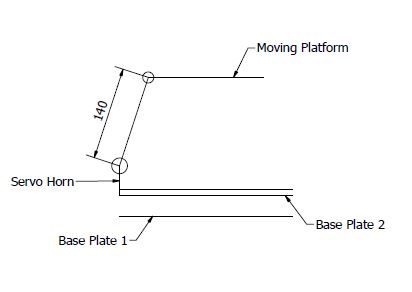
\includegraphics[width=0.6\linewidth]{Figures/Ideation}
	\caption[Ideation]{Ideation technique to obtain rod length}
	\end{figure}
\end{center}

\subsection{Sensing Rods Design - Shape}
Two options can be considered:
\begin{itemize}
\item Solid cylindrical rods
\item Hollow Cylindrical rods
\end{itemize}
From local suppliers, 10mm aluminium rods are available and economical. The rods are not hollow. From $\sigma = \frac{F}{A}$, where $\sigma$ - Stress, F - Axial Force on the leg and, A - Cross-sectional area, for the same amount of axial load, the hollow rod will experience more stress and consequently larger strains as compared to the solid rod. The rods are threaded at the ends for coupling with the spherical joints.

If solid rods are used, strain gauges of high sensitivity should be used.
\begin{center}
	\begin{figure}[H]
	\centering
	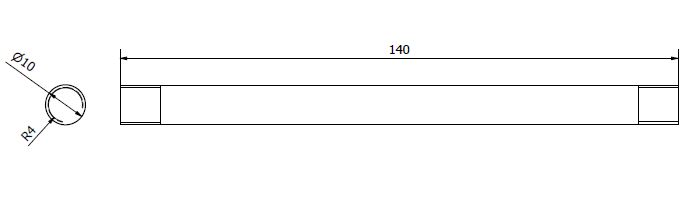
\includegraphics[width=0.8\linewidth]{Figures/Rod}
	\caption[Aluminium rod]{Aluminium rod}
	\end{figure}
\end{center}

\section{Test Flange and Strut}
The test flange will be used to hold the strut during wind tunnel testing. For optimum results, the reference axis is taken to be in the middle of the middle platform \cite {fernandes_design_nodate}. The flange will be fastened to the moving platform by use of bolts and nuts. Fasteners are more economical and easy to achieve as compared to welding. M6 or M8 nuts cab be used for this purpose.

The test flange should hold the strut for a considerable length in order to keep the rotation of the strut below certain predefined values and thus limiting torsion and bending behaviour of the strut during Wind Tunnel testing.
\begin{center}
	\begin{figure}[H]
	\centering
	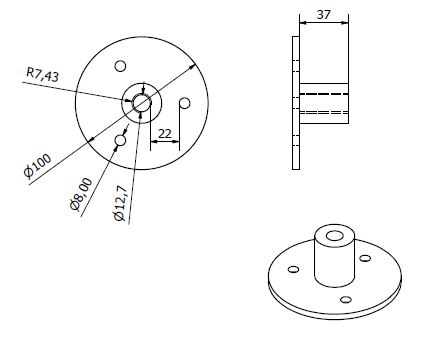
\includegraphics[width=0.75\linewidth]{Figures/Test}
	\caption[Test flange]{Test flange design}
	\end{figure}
\end{center}
The strut will go into the test section of the Wind tunnel at the Fluids lab in JKUAT. The strut should be long enough to position the model under testing in the middle of the test section. The strut will also be subjected to the flow forces in the wind tunnel. It should therefore be made of as small diameter as possible. A diameter 12.5mm of and a length of 400mm were considered, based on the Wind Tunnel set-up (Appendix).
\begin{center}
	\begin{figure}[H]
	\centering
	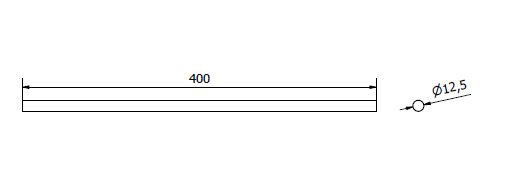
\includegraphics[width=0.75\linewidth]{Figures/Strut}
	\caption[Strut]{Strut}
	\end{figure}
\end{center}

\section{Spherical Joints}
For the 6-6 type, both platforms have six vertices and
the connections between the sensing bars and the platforms is made by simple spherical joints. Single spherical joints are chosen because they are easy to manufacture and they eliminate the issues of interference between sensing bars when double spherical joints are used \cite{fernandes_design_nodate}. 

Connection with spherical joints also prevents the torsion and bending phenomena in the bars when subjected to axial forces \cite{fernandes_design_nodate}.

Spherical joints can be obtained from online stores. One such store is RS Components Africa. Options of spherical joints to choose from include:
\begin{itemize}
\item Ball and socket joint M5
\item Ball and socket joint M6
\item Ball and socket joint M8
\item Ball and socket joint M10
\end{itemize}
Based on the diameter of the available aluminium rods, Ball and socket joint M10 is selected.
\begin{center}
	\begin{figure}[H]
	\centering
	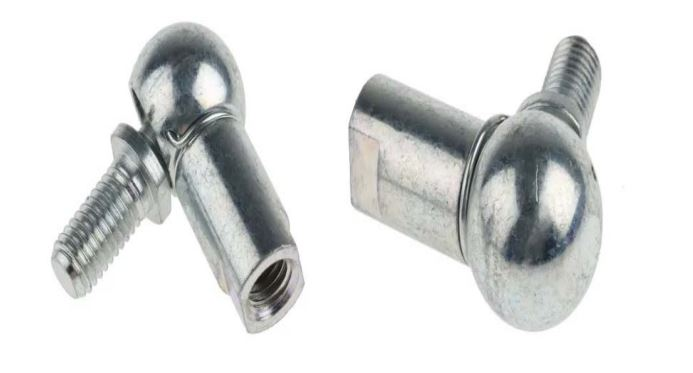
\includegraphics[width=0.6\linewidth]{Figures/Spherical}
	\caption[Spherical Joint]{Spherical Joint available from RS Components Africa \cite{datasheet_spherical}}
	\end{figure}
\end{center}
The following dimensions are provided by the manufacturer:
\begin{center}
	\begin{figure}[H]
	\centering
	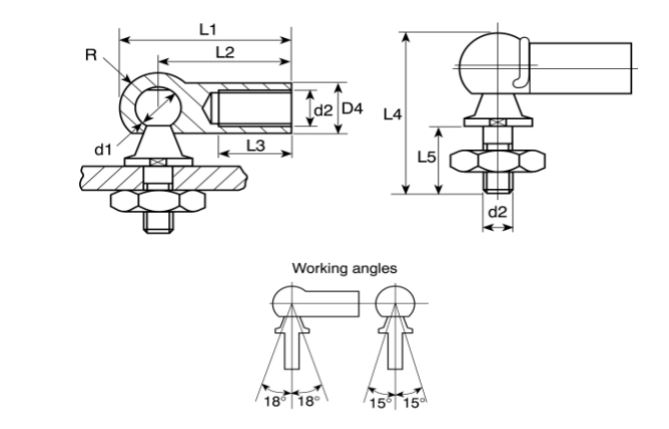
\includegraphics[width=0.8\linewidth]{Figures/Spherical Dimensions}
	\caption[Spherical Joint Dimensions]{Spherical Joint Dimensions \cite{datasheet_spherical}}
	\end{figure}
\end{center}
\begin{table}[H]
\caption{Spherical Joint Dimensions}
\end{table}
\begin{tabular}{|l|l|l|l|l|l|l|l|l|l|l|l|}
\hline
\textbf{Size(mm)}& \textbf{D1}& \textbf{D2}&\textbf{ D4}& \textbf{L1}& \textbf{L2}& \textbf{L3}& \textbf{L4}& \textbf{L5}& \textbf{R} & \textbf{A/F} & \textbf{min pull-off Force(N)}\\
\hline
10 & 16 & M10 & 16 & 47 & 35 & 15.5 & 47.5& 20 & 12 & 13 & 80\\
\hline
\end{tabular}

\paragraph{}

The Spherical joint was done on Autodesk Inventor and included in the Stewart Platform Assembly.
\begin{center}
	\begin{figure}[H]
	\centering
	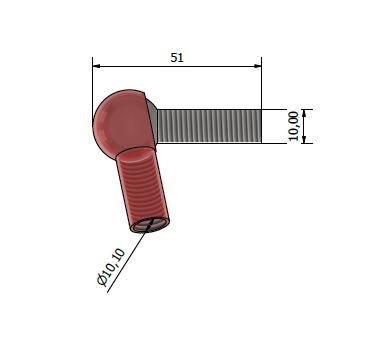
\includegraphics[width=0.5\linewidth]{Figures/Spherical CAD}
	\caption[Spherical Joint CAD]{Spherical Joint as designed on Autodesk Inventor}
	\end{figure}
\end{center}

\section{Electromechanical Design}
Two methods of actuation are popular with Stewart platforms:
\begin{itemize}
\item Linear actuators
\item Use of motors
\end{itemize}
Whereas linear actuators are relatively easy to control, they are very expensive. Thus the choice of motors.
\subsection{Servo Horn}
This will provide the connection between the motor and the spherical joints hence the aluminium rods. An 8mm hole on one end for mounting the spherical joint and another hole 8.5mm that will allow coupling with the servo arm bush of 8.6mm. The 1mm gap ensure tight fitting.
\begin{center}
	\begin{figure}[H]
	\centering
	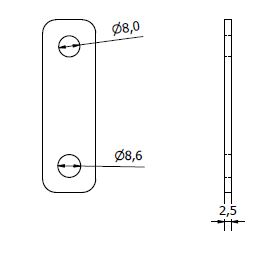
\includegraphics[width=0.6\linewidth]{Figures/Horn}
	\caption{Servo horn}
	\end{figure}
\end{center}

\subsection{Motor Selection}
One parameter was considered in our motor selection i.e. torque required. From the Autodesk Inventor design environment, the mass of the moving platform and mechanical couplings was 2.6kg. Each motor is supposed to move a minimum mass of 0.177kg. Using a servo horn of distance 45mm centre-to-centre, and Distance = $ \pi $ D, then:
\begin{equation}
Torque = (0.1777 \times 9.81)\times \frac{141.37}{1000} = 0.246 N\cdot m
\end{equation}
Motors of minimum torque of 0.2 N $\cdot m$ were considered. But for control considerations, only stepper motors and servo motors were shortlisted. Servo motor was considered over Stepper motor because they are cheaper. Also, we are only interested in 0 - 180 degrees positions.

The Servo motor \textbf{TowerPro SG5010} is suitable for this project. The specifications provided by the manufacturer are as follows:

\begin{table}[!h]
\caption[Motor Specifications]{TowerPro SG5010 Specifications}
\end{table}
\begin{center}
\begin{tabular}{|l|l|}
\hline
\textbf{Model}& TowerPro SG5010\\
\hline
\textbf{Operating Voltage} & 4.8V - 6.6V\\
\hline
\textbf{Operating Speed @ 4.8V} & 0.20sec/60$^{\circ}$\\
\hline
\textbf{Operating Speed @ 6.6V}& 0.16sec/60$^{\circ}$\\
\hline
\textbf{Stall torque @ 4.8V} & 5.5 kg-cm or 0.54 N $\cdot$ m\\
\hline
\textbf{Stall torque @ 6.6V} & 6.5 kg-cm or 0.64 N $\cdot$ m\\
\hline
\end{tabular}
\end{center}

\section{Design of the Force Sensor}
The force sensor module will be used to measure the force and moments from the aerodynamic loads applied on model being tested in the wind tunnel. The forces to be measured are the drag, lift and thrust as well as associated moments. For this subsystem two possible conceptual designs are to be considered:
\begin{itemize}
\item External force sensor
\item Stewart Platform as a force sensor
\end{itemize}
\subsection{External Force Sensor}
In this case it would require at least 3 orthogonally positioned load cells measuring each force component. Each load cell would be mechanically linked to the model such that forces experienced on each axis are measured by each load cell. 
\begin{center}
	\begin{figure}[H]
		\centering
		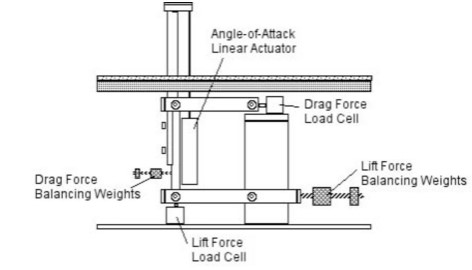
\includegraphics{Figures/modBal}
		\caption[Diagram of a force balance]{Diagram of a force balance \cite{post_force_2010}}
	\end{figure}
\end{center}
This configuration is, however, bulky since it requires an additional external system for force measurements in addition to the Stewart platform for positioning the model. This is however complemented by the simplicity in calibration of the load cells and does not require a complex force transformation matrix and other issues with force amplification created by the use of an integrated system.
\subsection{Stewart Platform as a force sensor}
In this configuration the Stewart platform legs are used as force sensors by attaching strain gauges on the legs of platform. Similar work has been done by \cite{ferreira2015design} without the use of actuators as is proposed in this project. Using the Stewart platform as a force sensor requires the actuators to be locked with zero degrees of freedom.

Four strain gauges are required for each leg for a full Wheatstone bridge configuration. 
\begin{center}
	\begin{figure}[H]
		\centering
		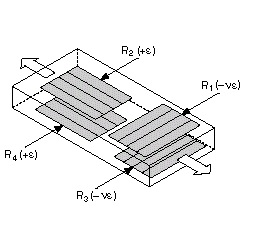
\includegraphics{Figures/loadConf}
		\caption[Strain Gauge Configuration]{Strain Gauge Configuration \cite{noauthor_measuring_nodate}}
	\end{figure}
\end{center}
In this case, as shown in figure 3.8.2, the load cells are able to measure the axial strain on each leg. R1 and R3 are active strain gauges measuring the compressive Poisson effect (–νe). R2 and R4 are active strain gages measuring the tensile strain (+e). The output generated from the Wheatstone bridge is then amplified and read to determine the strain on each leg.
In the case of this project, a full bridge strain gauge sensor with each strain gauge orthogonally positioned allowing for elimination of noise and measurement of the strain axially on each rod is used.

\paragraph{Force measurement Circuit}
The output excitation of the Wheatstone bridge needs to be amplified as it results in low outputs. An analogue to digital converter is also required for the analogue to digital converter. Some considerable options are the HX711 or the AD7193 converters which may be used as digital to analogue converters. The AD7193 is designed for high precision and has a delta sigma filter to remove noise from measurements.  However the AD7193 was not used due to it's high cost compared to the HX711 regardless of the advantage it offers with serial peripheral Interface communication allowing for multiple modules on the same bus.

The connection of the AD7193 to the microcontroller will be via Serial Peripheral Interface (SPI). The configuration is as shown in figure 3.8.3:
\begin{center}
\begin{figure}[H]
\centering
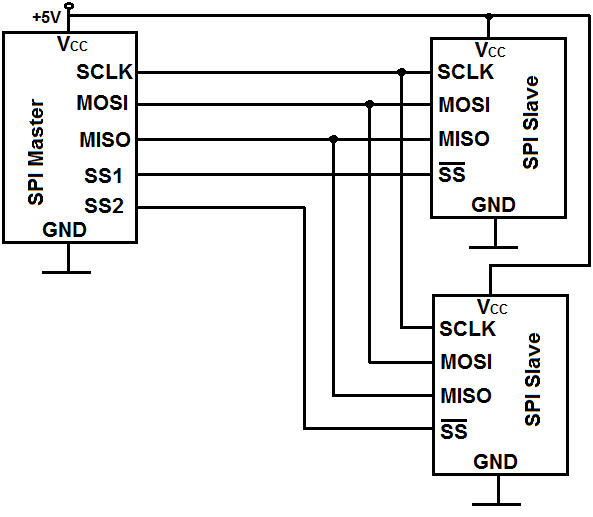
\includegraphics[width=0.55\linewidth]{Figures/SPI}
\caption[SPI configuration]{SPI configuration}
\end{figure}
\end{center}
In this configuration the when the chip select pin of an amplifier is set to low, the microcontroller is able to obtain data from that strain gauge. This configuration allows for a four wire interface to connect to six strain gauge sensors and obtain measurements.

The HX711 however allows for the I2C like communication via two wires (serial clock (SCL) and Serial Data (SDA)). They however do not have hardware addresses thus many pins are required for the interface, This can however be remedied by the use of a shared SCL between each of the amplifier modules reducing the overall number of pins required to interface.

\paragraph{Force transformation matrix} 
In such a case the forces experienced at the top of the platform are distributed between the 6 legs and as result, a force transformation matrix is required to resolve the forces applied on each axis as measured by each load cell on each leg. 

If the platform is acted upon by an external wrench {$\vec{F}_e, \vec{M}_e$}, for static equilibrium of the body, the external wrench is statically balanced by the six leg forces of the Stewart platform. Representing the unit vector $\hat{I}_i$ along the i-th leg with respect to B, the leg force is given  by $\hat{I}_if_i$. Considering the force equilibrium of the platform along  three mutually perpendicular directions in B(XYZ), the following force equations can be obtained as in \cite{dwarakanath_design_2001}:

\begin{equation}
	(F_e)_x = f_1I_{1x} + f_2I_{2x} + f_3I_{3x} + f_4I_{4x} + f_5I_{5x} + f_6I_{6x}
\end{equation}
\begin{equation}
	(F_e)_y = f_1I_{1y} + f_2I_{2y} + f_3I_{3y} + f_4I_{4y} + f_5I_{5y} + f_6I_{6y}
\end{equation}
\begin{equation}
	(F_e)_z = f_1I_{1z} + f_2I_{2z} + f_3I_{3z} + f_4I_{4z} + f_5I_{5z} + f_6I_{6z}
\end{equation}
where $(F_e)_x$, $(F_e)_y$ and $(F_e)_z$ are the external forces on the platform along three mutually perpendicular directions x, y and z of the frame B, respectively.

The moment due to the forces $\hat{I}_if_i$ about the origin of B is $(\vec{b}_i x \hat{I}_i)f_i$. Considering the moment equilibrium about x, y and z axes of B, the following moment equations can be obtained as in \cite{dwarakanath_design_2001}:

\begin{equation}
	(M_e)_x = f_1(\vec{b}_1 x \hat{I}_1)_x + f_2(\vec{b}_2 x \hat{I}_2)_x + f_3(\vec{b}_3 x \hat{I}_3)_x + f_4(\vec{b}_4 x \hat{I}_4)_x + f_5(\vec{b}_5 x \hat{I}_5)_x + f_6(\vec{b}_6 x \hat{I}_6)_x
\end{equation}
\begin{equation}
	(M_e)_y = f_1(\vec{b}_1 x \hat{I}_1)_y + f_2(\vec{b}_2 x \hat{I}_2)_y + f_3(\vec{b}_3 x \hat{I}_3)_y + f_4(\vec{b}_4 x \hat{I}_4)_y + f_5(\vec{b}_5 x \hat{I}_5)_y + f_6(\vec{b}_6 x \hat{I}_6)_y
\end{equation}
\begin{equation}
	(M_e)_z = f_1(\vec{b}_1 x \hat{I}_1)_z + f_2(\vec{b}_2 x \hat{I}_2)_z + f_3(\vec{b}_3 x \hat{I}_3)_z + f_4(\vec{b}_4 x \hat{I}_4)_z + f_5(\vec{b}_5 x \hat{I}_5)_z + f_6(\vec{b}_6 x \hat{I}_6)_z
\end{equation}

where $(M_e)_x$, $(M_e)_y$ and $(M_e)_z$ are the external moments on the platform  about the three coordinate axes of B. Combining the equations the relationship between the external wrench and the forces experienced by the legs can be expressed as follows:
\begin{equation}
	$$
\begin{Bmatrix}
	\vec{F}_e \\
	\vec{M}_e \\
\end{Bmatrix} = [H]\{F\}
$$
\end{equation}


\section{Velocity Measurement}
An important part in wind tunnel measurements is the measure of pressure at specific points in the wind tunnel and computing the corresponding air speed. This is achieved by the use of a pitot probe. 
\begin{center}
\begin{figure}[H]
\centering
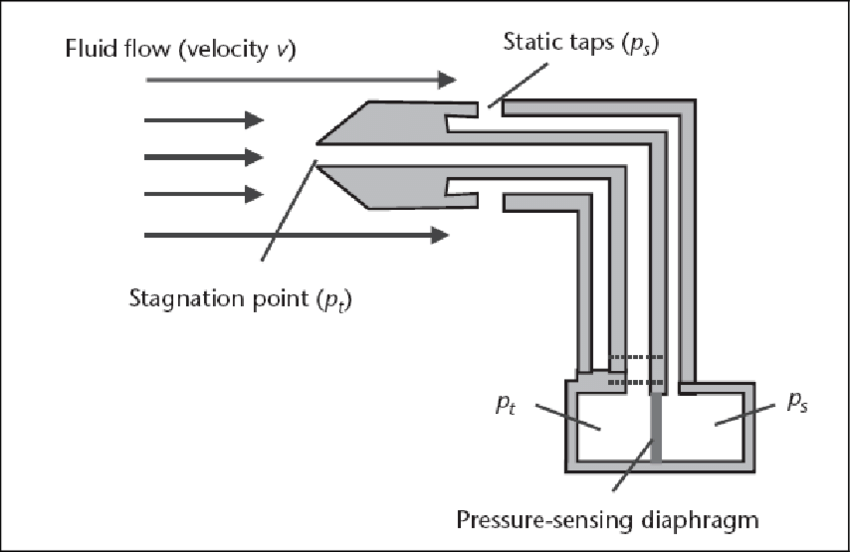
\includegraphics[width=0.6\linewidth]{Figures/pitot}
\caption[Pitot-static tube]{Pitot-static tube \cite{viquerat_continuous_2006}}
\end{figure}
\end{center}
For steady flow of an incompressible fluid for which viscosity can be neglected, the fundamental equation has the form:

\begin{equation}
	v = \sqrt{\frac{2(P_{0} - P)}{\rho}}
\end{equation}

Where V is the speed of the fluid, P0 is the total, also called the stagnation, pressure at that point of measurement, and p is the static pressure at the same point.

Three pitot probes are to be used in the wind tunnel i.e. in the test section, intake and diffuser sections.

Module communicates to the microcontroller using a TTL to RS485. Each module is individually addressable further simplifying the interface as shown in figure 3.9.2:
\begin{center}
\begin{figure}[H]
\centering
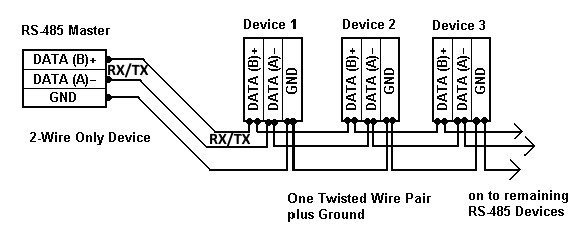
\includegraphics{Figures/modbus}
\caption[RS485 communication]{RS485 communication}
\end{figure}
\end{center}

\section{Design of Human Machine Interface}
The purpose of the interface is to enable control of the platform position as well as to obtain measured data from the strain gauges and pitot tubes. 
The general layout is as shown in the figure below:
\begin{center}
\begin{figure}[H]
\centering
\includegraphics{Figures/Interface}
\caption[Human Machine Interface]{Human Machine Interface}
\end{figure}
\end{center}

The primary interface between the microcontroller is wirelessly via web sockets utilizing the User Datagram Protocol (UDP) interface. This allows for high speed low latency communication without need for a wired connection. It also allows for bidirectional transfer of information thus allowing for both control input and output of measured values. The interface is to enable the abstraction of data acquisition and actuator control to a simple interaction with buttons and other visual interfaces available in a computer program.

The decoupling of the microcontroller and the program to be hosted on the desktop allows for advanced data processing such as application of filters and resolving measurements into usable information. It also allows for the use of more powerful processor and high level programming languages to more effectively perform complex calculations without taking a toll the sensor sampling rate that would occur with on board processing in the microcontroller.
\begin{center}
	\begin{figure}[H]
	\centering
	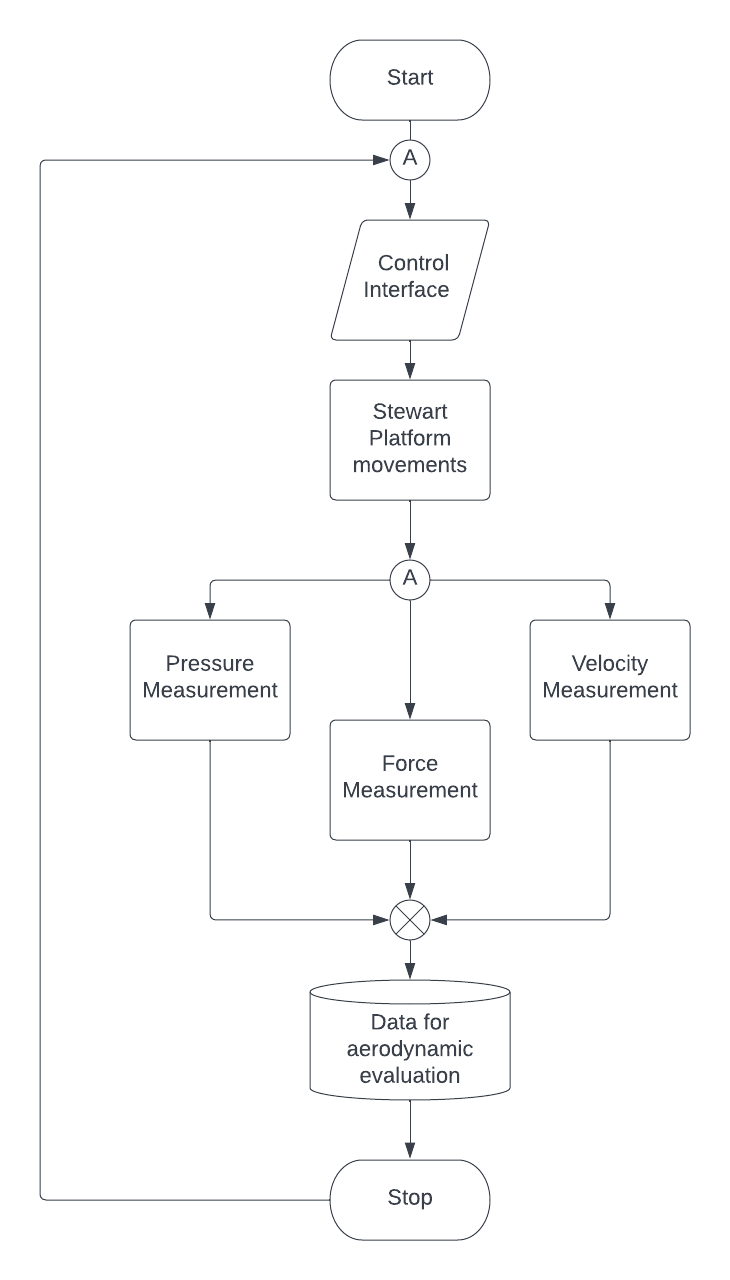
\includegraphics[width=0.7\linewidth]{Figures/Fig14}
	\caption[Control Algorithm]{Control Algorithm for the Stewart Platform with Force Measurement}
	\end{figure}
\end{center}
\section{Printed Circuit Board Design}
This section looks at the design of the circuits used to power and get readings from the sensors and control the actuators.

\subsection{Microcontroller}
The main requirement for this is the need for wireless communication via WIFI and large number of I/O interface at cost effective rate. This brings down the options to the ESP32 and Raspberry Pi RP2040. Both are dual core devices which are feature rich however the raspberry rp2040 only has 28 I/O pins while the ESP32 has 34 pins and due to this the ESP 32 was chosen. 
\begin{center}
	\begin{figure}[H]
	\centering
	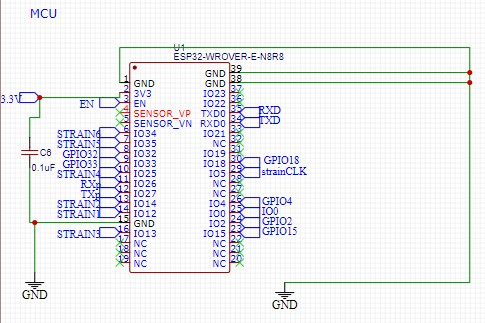
\includegraphics{Figures/mcu}
	\caption[Microcontroller]{Microcontroller}
	\end{figure}
\end{center}

\subsection{Power Supply}
The power supply chosen is a AC/DC power converter. Since the highest voltage required is 12 volts. This also used as the highest power supply to the PCB.

Both 5 and 3.3 volts are required in the PCB for other peripherals. To this end a buck converter and linear converter are used for 5 ad 3.3 volts respectively.

\begin{center}
	\begin{figure}[H]
	\centering
	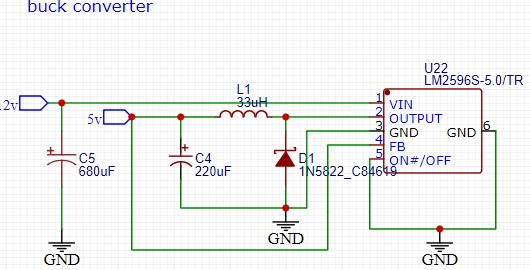
\includegraphics{Figures/buck}
	\caption[Buck converter]{Buck Converter 12V to 5v}
	\end{figure}
\end{center}

\begin{center}
	\begin{figure}[H]
	\centering
	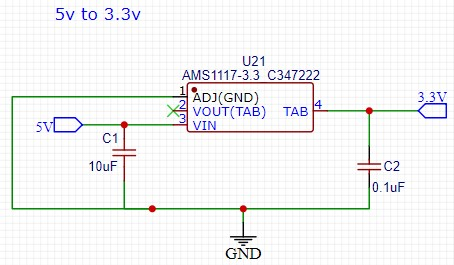
\includegraphics{Figures/5233}
	\caption[Linear Voltage Converter]{Linear level converter 5V to 3.3v}
	\end{figure}
\end{center}

The linear converter dissipates the energy loss though heat while buck converter is through switching.

\subsection{Servo Control}
Since the microcontroller used (ESP32) is based on 3.3V logic. There is a need for 5V logic to control the servos and thus a bidirectional logic level converter is utilized which leverages an internal drain N-channel MOSFET. 
\begin{center}
	\begin{figure}[H]
	\centering
	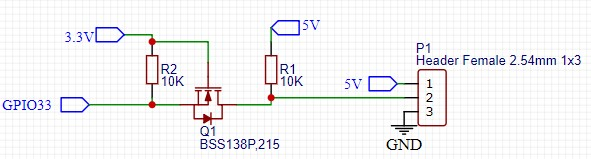
\includegraphics{Figures/logik}
	\caption[Bidirectional Logic Level converter]{Bidirectional Logic Level converter}
	\end{figure}
\end{center}
